%\tablesofcontent

\section{Industrial contexts and results}

\subsection{Industrial environnment}
\begin{frame}{Programmation environnement}

  \begin{multicols}{2}
    \begin{figure}[H]
      \centering
      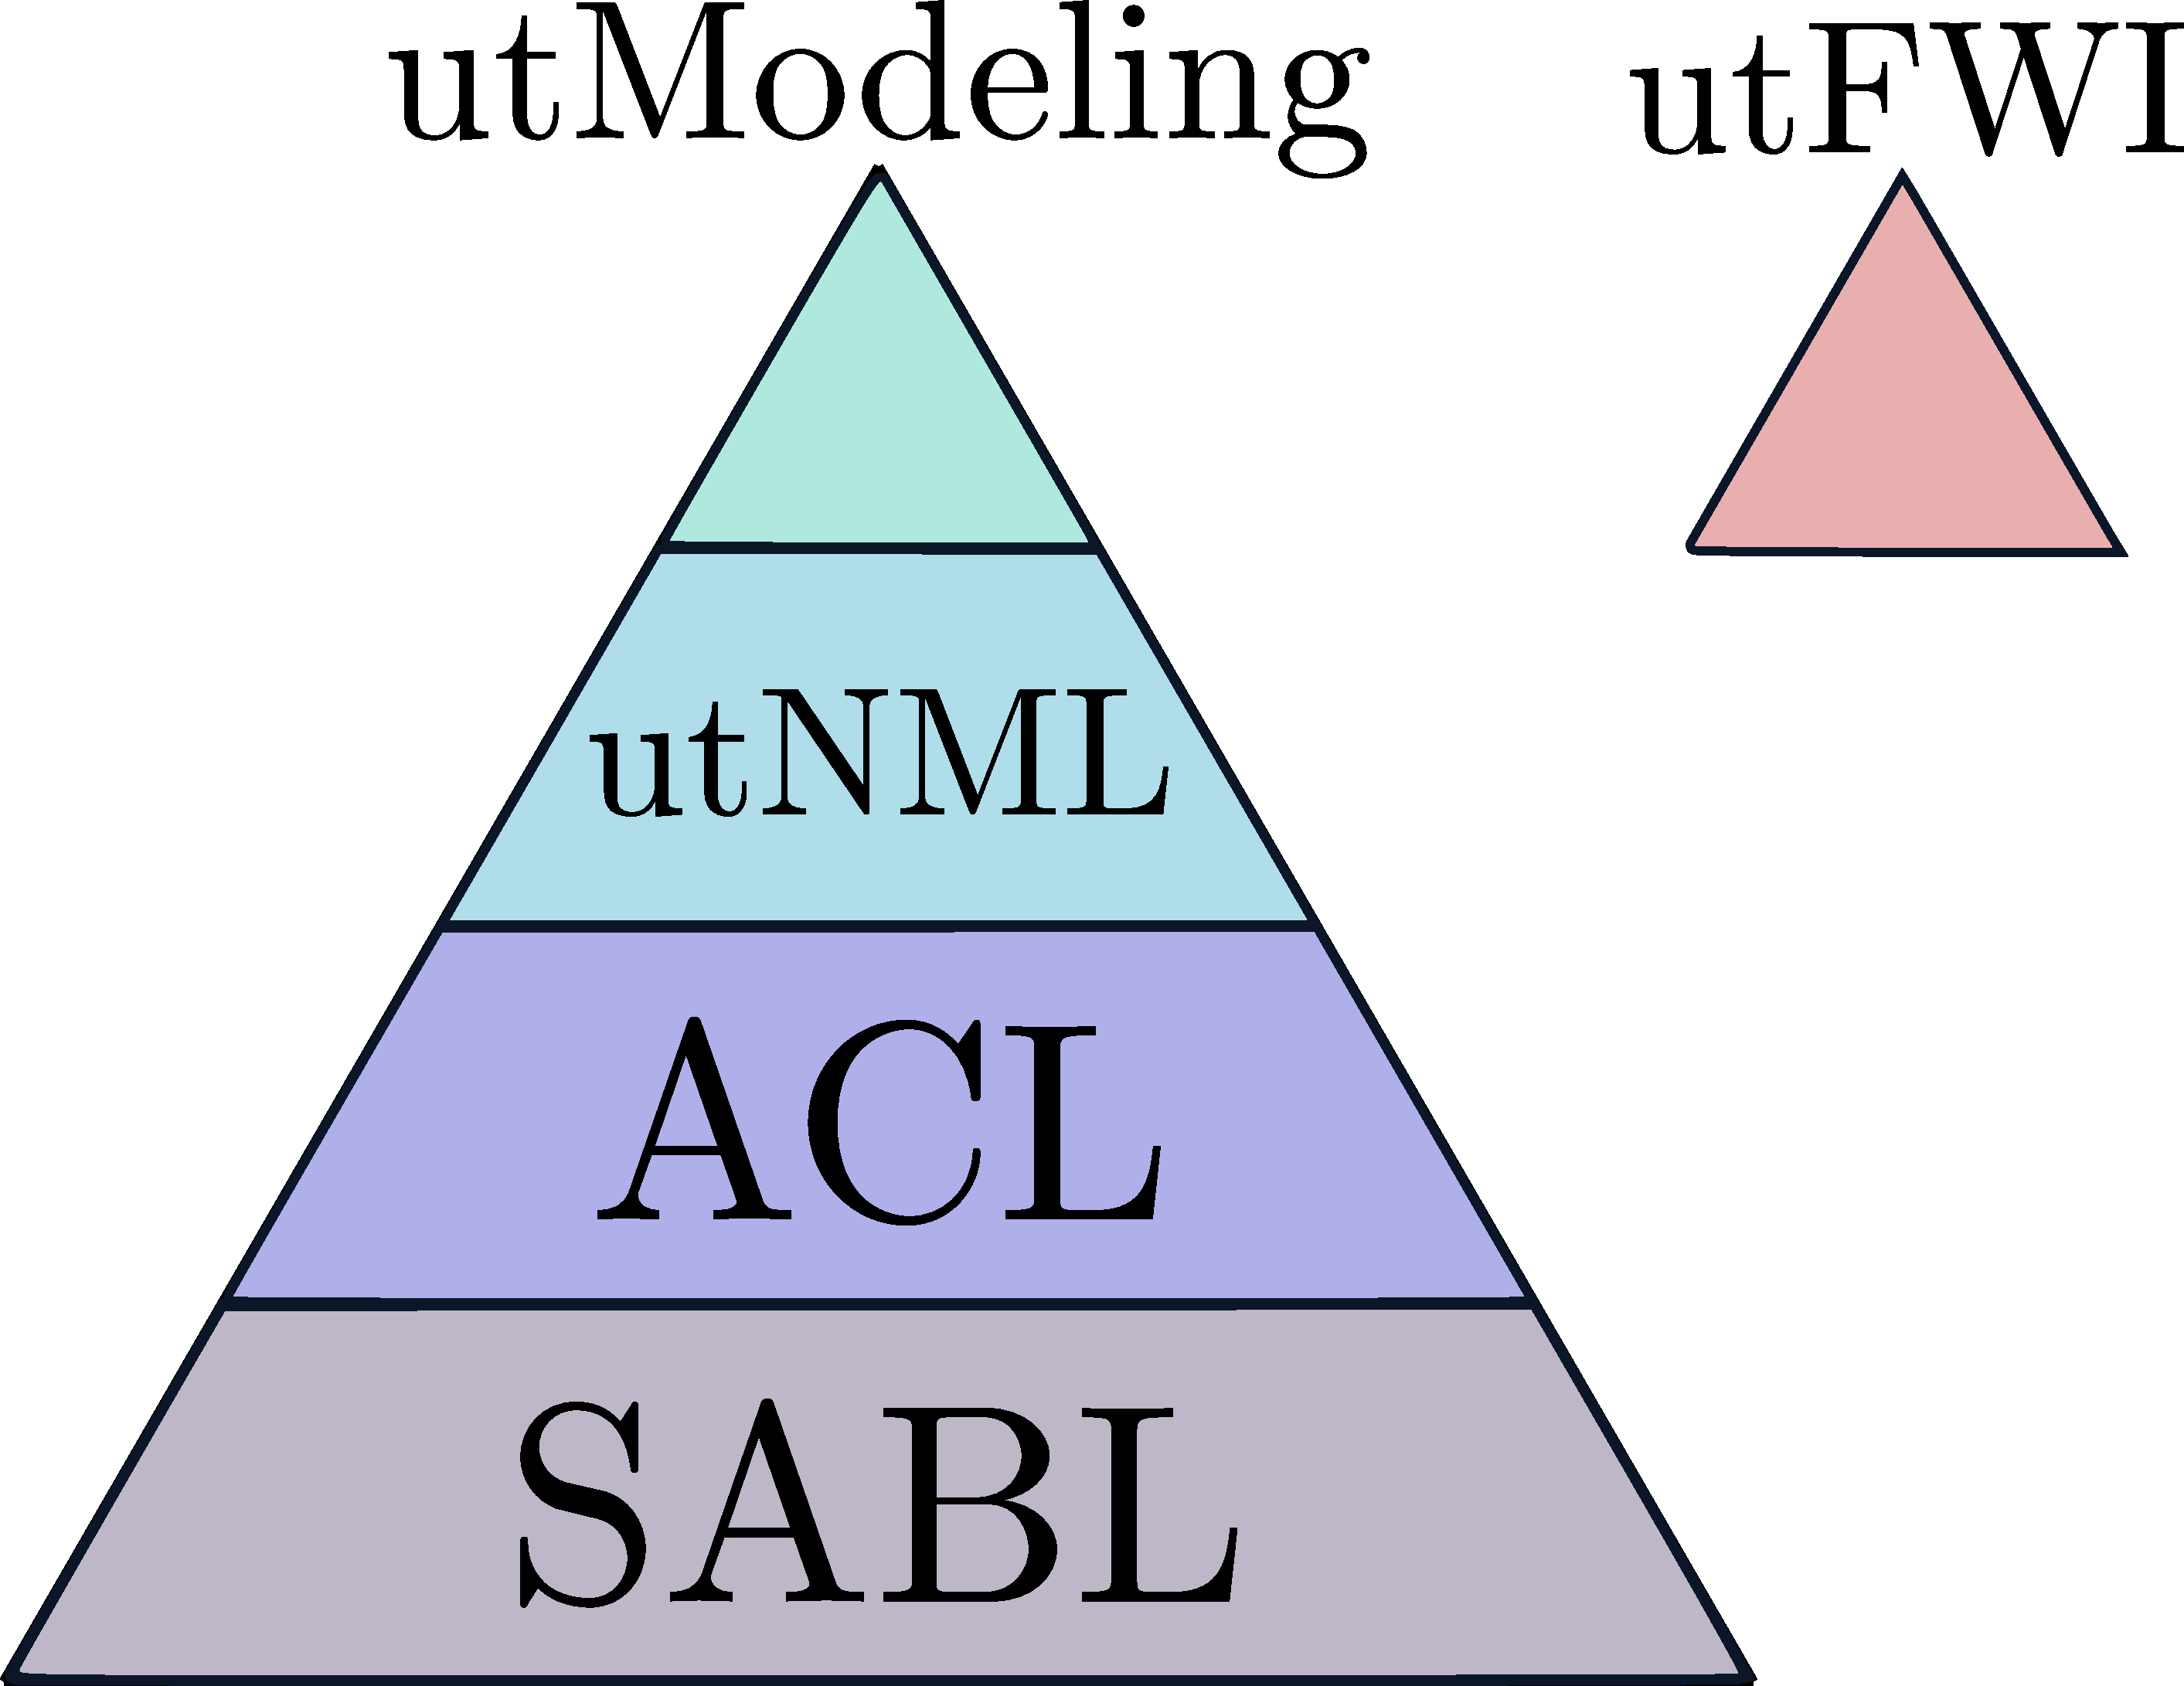
\includegraphics[scale=0.12]{image/carbon.pdf}
      \caption*{Illustration of the hierarchical Total's environnement.}
      \label{carbon}
    \end{figure}

    \columnbreak

    \begin{itemize}
      \small
    \item<2-> \textbf{SABL}: Seismic Application Base Library (Seismic acquisition + Parallelism)
    \item<3-> \textbf{ACL}: Application Core Library  (Discrete operator + Domain decomposition)
    \item<4-> \textbf{utNML}: Unstructured Time-domain Numerical Methods Library (Propagators + Models + Seismic Data management)
    \item<5-> \textbf{utModeling}: Unstructured Time-domain Modeling (Main application to perform the modelling)
    \end{itemize}
  \end{multicols}

\end{frame}


\subsection{Parallelism}
\begin{frame}{Parallelism}{Two levels of parallelism}

  \begin{overprint}
    \onslide<2>
  \begin{figure}[H]
    \centering
    
\includegraphics[scale=0.15]{image/partition.png}
    \caption{$nb\_domain=10$ cores to solves one forward problem (shot)\footcite{karypis1997parmetis}.}
    \label{partition}
  \end{figure}
      \onslide<3>
\begin{figure}[H]
  \centering
  \includegraphics[scale=0.055]{image/partition_cluster.pdf}
  \caption*{Illustration of shot parallelism for gradient computation.}
  \label{partition_cluster}
\end{figure}

$nb\_cores = nb\_domain \times nb\_cluster$

  \end{overprint}
  \end{frame}

\subsection{Results}
\begin{frame}{Results}{TO DO}

  \begin{itemize}
  \item 1 slide results marmousi
  \item 1 slide results overthrust 2D
  \item 1 slide results sigsbee
  \item 1 slide results Seam Foothills reduced 3D
  \item 1 slide results Overthrust 3D
  \end{itemize}
\end{frame}
